
\documentclass[11pt,serif,aspectratio=169]{beamer}

% Set the margins to be something normal.
% \usepackage[margin=1in]{geometry}

% Fun lists!
\usepackage{enumitem}
\usepackage{textcomp}
\setitemize{label=\textrightarrow, itemsep=0pt}

% Math symbols.
\usepackage{amsmath, amssymb, amsfonts, tikz,mathtools}

% No indents.
\setlength\parindent{0pt}
\setlength\parskip{1em}

\newcommand{\inverse}[1]{#1^{-1}}


% Nice fonts :)
%\usepackage{tgschola}
\usefonttheme[onlymath]{serif}

\begin{document}

	\begin{frame}
		Suppose that $$f(x) = 2x^2$$ and $$g(x) = x^3.$$
		We are going to find the \textbf{volume of the solid generated by rotating these curves} using \textbf{two different methods.}
	\end{frame}
	
	\begin{frame}
		\center{\Large{\bf the disk and washer methods}}
	\end{frame}
	
	\begin{frame}
		The \textbf{disk method} is based on \textbf{finding the areas of infinitely thin donuts, or ``washers,''} and adding those areas up.
	\end{frame}
	
	\begin{frame}
		To add those areas up, we use \textbf{an integral}. If we
		\begin{enumerate}[label=(\roman*)]
			\item know our \textbf{bounds of integration},
			\item are \textbf{rotating our solid around the $x$ axis}, and
			\item \textbf{have two functions} $f_{\text{top}}$ and $f_{\text{bottom}}$,
		\end{enumerate}
		our integral to find the volume is $$ V_{\text{washer}} = \int_a^b \pi(\underbrace{f_{\text{top}}(x)}_{\mathclap{\text{radius of outer circle}}})^2 -\pi (\overbrace{f_{\text{bottom}}(x)}^{\mathclap{\text{radius of inner circle}}})^2 dx,$$ which can be re-written as $$ V_{\text{washer}} = \pi \int_a^b (\underbrace{f_{\text{top}}(x)}_{\mathclap{\text{radius of outer circle}}})^2 - (\overbrace{f_{\text{bottom}}(x)}^{\mathclap{\text{radius of inner circle}}})^2 dx$$
		\footnotesize{What happens if we don't have two functions?}
	\end{frame}
	
	\begin{frame}\centering
		Let's apply it.
	\end{frame}
	
	\begin{frame}
		We set $$ f(x) = f_\text{outer}(x), \ \ \ g(x) = f_\text{inner}(x)$$ (because $f$ is ``on top'' of $g$)
		and find where the curves intersect --- that is, where the \textbf{curves hit the same value.} This gives us our \textbf{bounds of integration.}
	\end{frame}
	
	\begin{frame}
		\begin{align*}
			f(x) &= g(x) \\[1em]
			2x^2 &= x^3 \\
			2 &= \frac{x^3}{x^2} \\
			2 &= x
		\end{align*}
		so the curves intersect at the points $$ (2, f(2)) = (2, g(2)) = (2, 8) $$ and $$ (0, f(0)) = (0, g(0)) = (0, 0) $$
	\end{frame}
	
	\begin{frame}\centering\Large
		We will integrate from $x=0$ to $x=2$.		
	\end{frame}
	
	\begin{frame}
		Setting up our integral, we get	
		\begin{align*}
			V_\text{washer} &= \pi \int_0^2 f(x)^2 - g(x)^2 dx \\
			&= \pi \int_0^2 (2x^2)^2 - (x^3)^2 dx \\
			&= \pi \int_0^2 4x^4 - x^6 dx \\
			&= \left. \pi \left[\frac 45 x^5 - \frac 17 x^7 \right] \right|_0^2 \\
			&= \frac{256 \pi}{35}
		\end{align*}
	\end{frame}
	
	\begin{frame}\centering \Large \bf
		the shell method	
	\end{frame}
	
	\begin{frame}
		The \textbf{shell method} finds the \textbf{surface area of infinitely thin cylinders} and adds them up to find a volume. Recall that the surface area of a cylinder \textit{without a top or bottom} (like a straw) is $$ S = 2\pi \cdot r \cdot h $$ To add those areas up, we use \textbf{an integral} again.
	\end{frame}
	
	\begin{frame}
		If we
		\begin{enumerate}[label=(\roman*)]
			\item know our \textbf{bounds of integration},
			\item are \textbf{rotating our solid around the $x$ axis}, and
			\item \textbf{have two functions} $\inverse f_{\text{top}}$ and $\inverse f_{\text{bottom}}$,
		\end{enumerate}
		we have good information. However, we need to \textbf{change our perspective} --- if we are rotating around the $x$-axis, then \textbf{our cylinders are in terms of $y$.} (Why?)
	\end{frame}

	
	\begin{frame}
		\begin{figure}
			\centering
			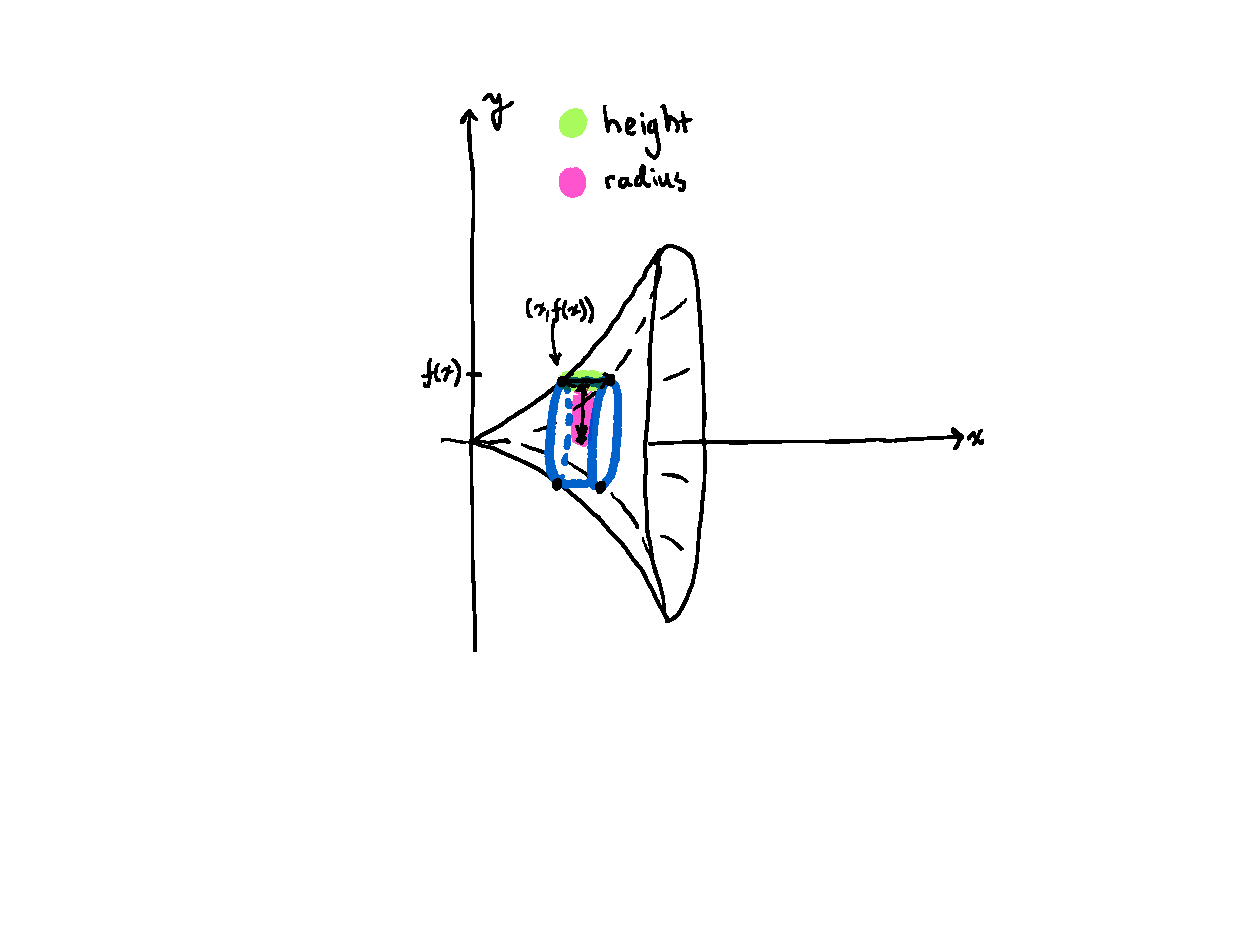
\includegraphics[height=0.9\paperheight]{x.pdf}	
		\end{figure}
	\end{frame}
	
	\begin{frame}
		\begin{figure}
			\centering
			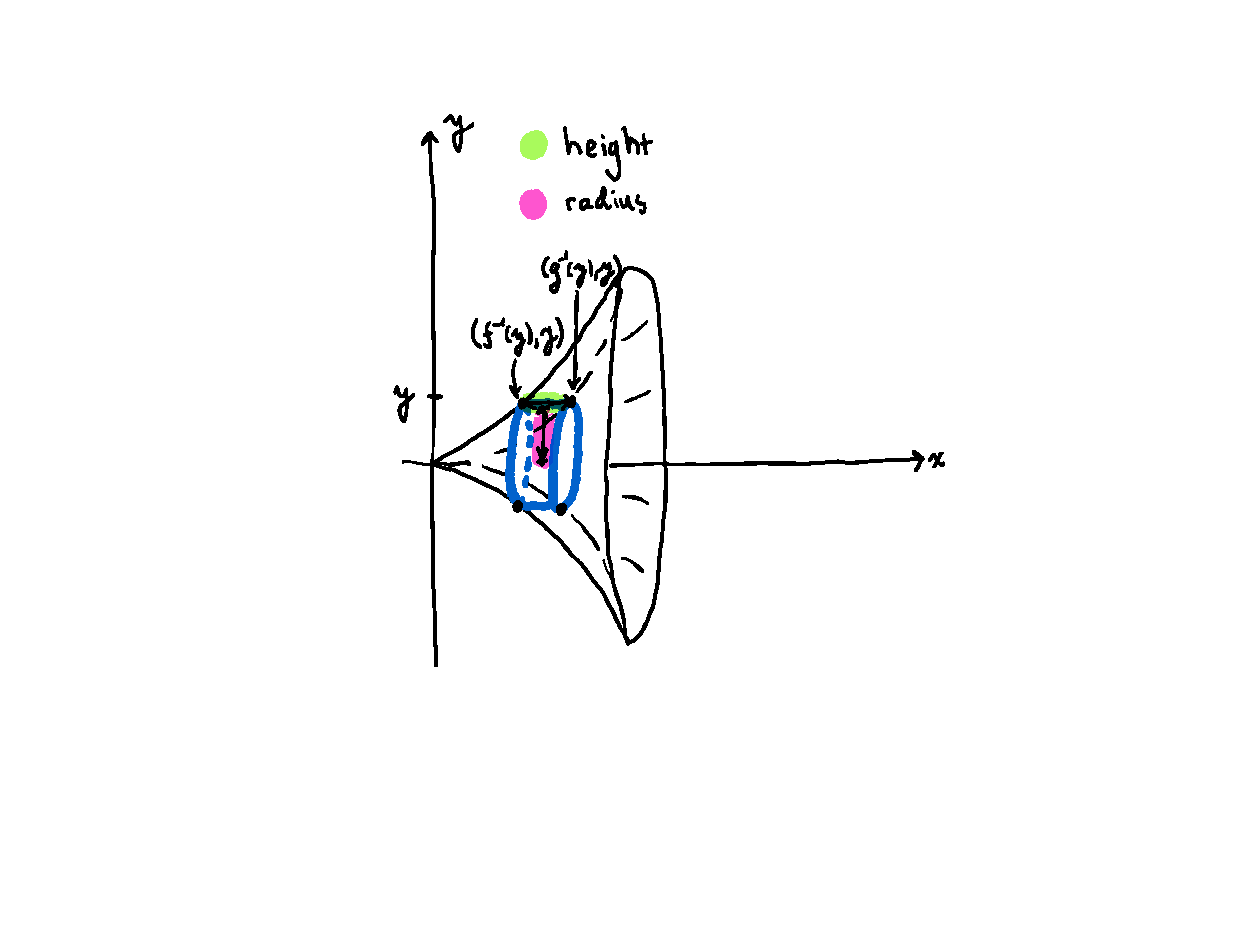
\includegraphics[height=0.9\paperheight]{y.pdf}	
		\end{figure}
	\end{frame}
	
	\begin{frame}
		We then find these \textbf{inverse functions} by setting up equations and \textbf{solving for $x$}:
		\begin{align*}
			y &= 2x^2 \\
			\frac y2 &= x^2 \\
			\sqrt{\frac y2} &= x = \inverse f(y), \\[1.5em]
			y &= x^3 \\
			\sqrt[3]y &= x = \inverse g(y)
		\end{align*}
	\end{frame}
	
	\begin{frame}
		Now, because the height and radius of our cylinders are in terms of $y$, we integrate with...	
	\end{frame}
	
	\begin{frame}
		Our integral is then $$ V_\text{shell} = \int_a^b 2 \pi \cdot \underbrace{y}_{\mathclap{\text{radius of cylinder}}} \cdot (\overbrace{\inverse f_\text{top}(y) - \inverse f_\text{bottom}(y)}^{\mathclap{\text{height of cylinder}}})\ dy,$$ which we can re-write as $$ V_\text{shell} = 2\pi \int_a^b y \cdot (\inverse f_\text{top}(y) - \inverse f_\text{bottom}(y))\ dy$$
	\end{frame}
	
	\begin{frame}
		Let's set up our integral!
		\begin{align*}
			V_\text{shell} &= 2\pi \int_a^b y \cdot (\inverse f_\text{top}(y) - \inverse f_\text{bottom}(y)) dy \\
			&= 2\pi \int_0^8 y \cdot \left(\sqrt[3]{y} - \sqrt{\frac y2} \right) dy \\
			&= 2\pi \left. \left[-\frac{\sqrt 2 y^{\frac 52}}{5} - \frac{3 y^{\frac 72}}{7} \right] \right|_0^8 \\
			&= \frac{256 \pi}{35},
		\end{align*}
		so we get the \textbf{same result}!
	\end{frame}
	
	\begin{frame}\Large \bf \centering
		questions?	
	\end{frame}


	
\end{document}
